\exer{1}

\setcounter{section}{0}

\vspace{0.25cm}


\section{Import}
\begin{prettyBox}{Import}{myblue}
\begin{itemize}
    \item \texttt{numpy} : Les fonctions mathématiques prédéfinies, et \texttt{linspace} pour créer  
        les vecteur des coordonnées x de chaque fonctions.  
    \item \texttt{matplotlib} : Dessine les graphes.  
    \item \texttt{collections} : Crée une nouvelle structure avec \texttt{namedtuple}.  
\end{itemize}
\end{prettyBox}
\vspace{0.5cm}
\lstinputlisting[style=pythonstyle, firstline = 1,lastline=3,basicstyle= \ttfamily\scriptsize]{Exercices/EX1/ex1.py}

\vspace{1cm}

\section{Définition Des Fonctions Mathématiques}
\lstinputlisting[style=pythonstyle, firstline = 7,lastline=17,basicstyle= \ttfamily\scriptsize]{Exercices/EX1/ex1.py}

\vspace{1cm}
\section{Génération des Vecteurs}
\lstinputlisting[style=pythonstyle, firstline = 50,lastline=58,basicstyle= \ttfamily\scriptsize]{Exercices/EX1/ex1.py}

\newpage
\section{Nouvelle Structure root}
\begin{prettyBox}{root}{myblue}
On a créé une nouvelle structure en utilisant \texttt{namedtuple} root. Elle représente 
les racines pour \( f(x) = 0 \) et possède trois attributs :
\begin{itemize}
    \item \textbf{position} : coordonnée x de la racine
    \item \textbf{a} : extrémité gauche de l'intervalle auquel la racine appartient
    \item \textbf{b} : extrémité droite de l'intervalle auquel la racine appartient
\end{itemize}
\end{prettyBox}
\vspace{0.5cm}
\lstinputlisting[style=pythonstyle, firstline = 5,lastline=5,basicstyle= \ttfamily\scriptsize]{Exercices/EX1/ex1.py}

\vspace{1cm}

\section{Scatter}
\begin{prettyBox}{Scatter}{myblue}
\begin{itemize}
    \item \texttt{scatter\_single(rootElement, colorValue, marker)} : Dessine un point
        qui représente une racine pour \( f(x) \). Elle vérifie si les extrémités de l'intervalle de la racine 
        sont égales. Si oui, le label est : \(\alpha = a\), sinon \(\alpha \in [a,b]\). On utilise cette fonction
        si \( f \) admet une seule racine.
    \item \texttt{scatter\_many(rootElement, colorValue, index, marker)} : Dessine un point
        qui représente une racine pour \( f(x) \). Elle vérifie si les extrémités de l'intervalle de la racine 
        sont égales. Si oui, le label est : \(\alpha_{\text{index}} = a\), sinon \(\alpha_{\text{index}} \in [a,b]\). On utilise cette fonction
        si \( f \) admet plusieurs racines.
\end{itemize}
\textbf{Paramètres :}  
\begin{itemize}
    \item \textbf{rootElement} : de type \texttt{root}
    \item \textbf{colorValue} : couleur du marqueur
    \item \textbf{index} : indice de la racine
    \item \textbf{marker} : style du marqueur
\end{itemize}
\end{prettyBox}
\vspace{0.5cm}
\lstinputlisting[style=pythonstyle, firstline = 19,lastline=30,basicstyle= \ttfamily\scriptsize]{Exercices/EX1/ex1.py}

\newpage

\section{Draw}
\begin{prettyBox}{Draw}{myblue}
La fonction \texttt{draw()} dessine le graphe et les points des racines
grâce à la liste des racines \texttt{rootList} et aux fonctions \texttt{scatter} que nous avons précédemment définies, Et retourne la valeur de l’indice incrémenté de 1 pour la mettre à jour.\\[0.1cm]
\textbf{Paramètres :}  
\begin{itemize}
    \item \textbf{x} : Vecteur numpy des coordonnées \( x \)
    \item \textbf{y} : Vecteur numpy des coordonnées \( y \)
    \item \textbf{functionLabel} : Label de la fonction
    \item \textbf{colorValue} : Couleur du graphe
    \item \textbf{rootList} : Liste de racines de type \texttt{root}
    \item \textbf{index} : Indice du subplot
    \item \textbf{title} : Titre du graph
    \item \textbf{marker} (optionnel, valeur par défaut = \texttt{'o'}) : Style du marqueur pour les racines
\end{itemize}
\end{prettyBox}
\vspace{0.5cm}
\lstinputlisting[style=pythonstyle, firstline = 34,lastline=47,basicstyle= \ttfamily\scriptsize]{Exercices/EX1/ex1.py}

\vspace{1cm}
\section{Reste Du Code}
\lstinputlisting[style=pythonstyle, firstline = 59,basicstyle= \ttfamily\scriptsize]{Exercices/EX1/ex1.py}

\newpage
\section{Figure}
\begin{center}
    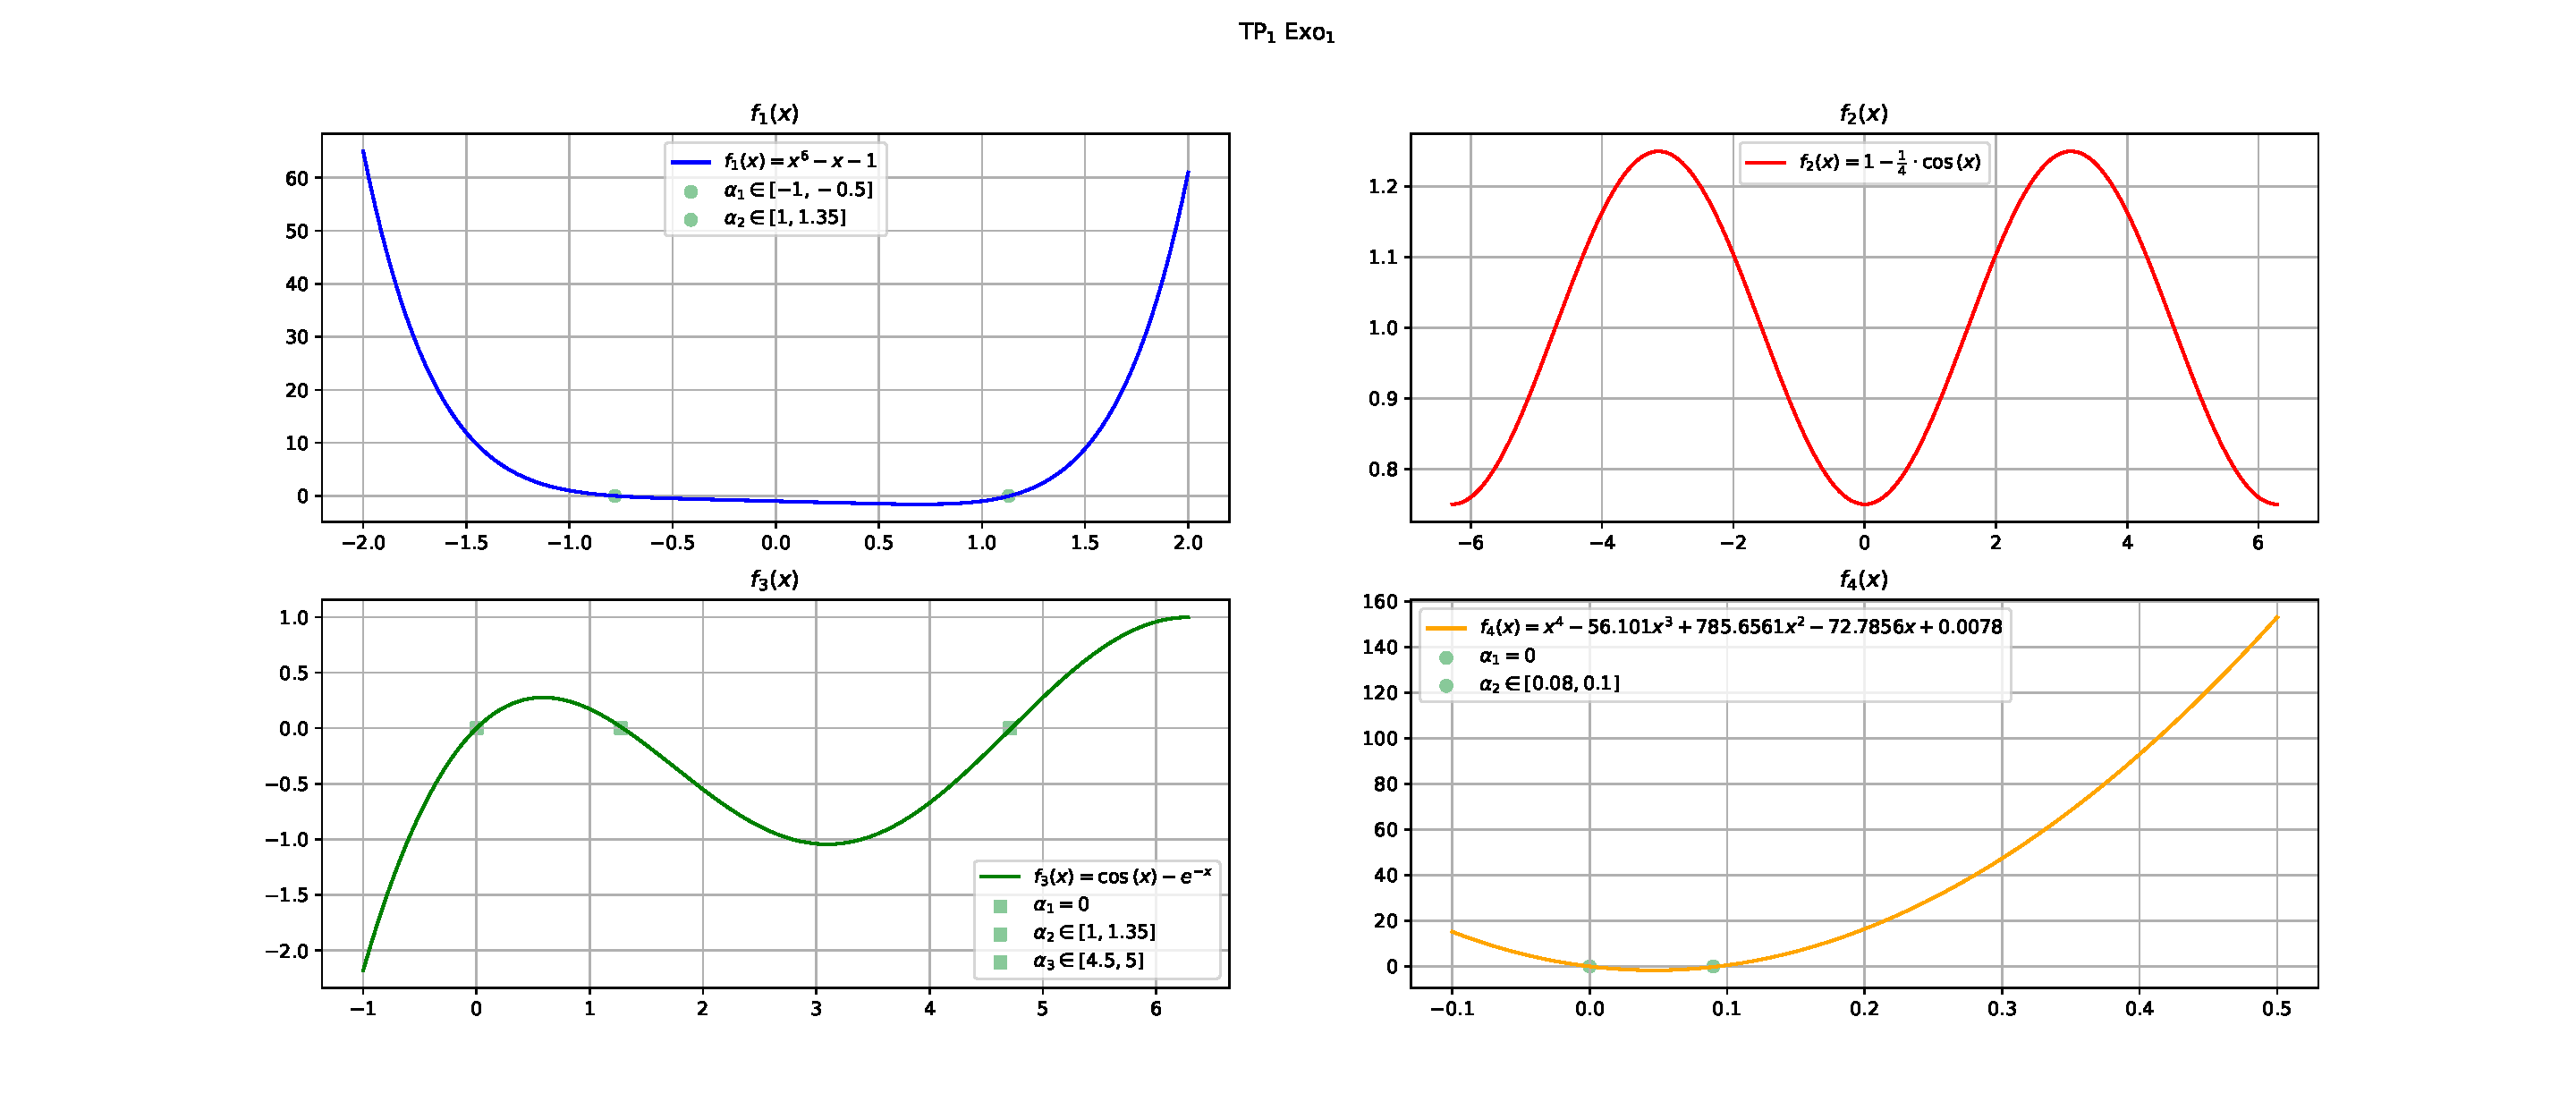
\includegraphics[height=0.35\textheight]{Exercices/EX1/fig.pdf}
\end{center}


